
\FloatBarrier
\subsection{Система Дуффинга} % _DUFF_

\LinkRef{
 duff: ASAU-12, 15. APIR-2009. DSMP-2016
}

\begin{equation}
 \ddot{x} + c_0 \dot{x} + \alpha x + \beta x^3 = u(t) ,
\label{atu:eq:duff}
\end{equation}
%
\begin{equation}
 m \ddot{x} + \nu \dot{x} + k_1 x + k_3 x^3 = F(t) ,
\label{atu:eq:duff_phys}
\end{equation}

Здесь $m$ -- масса объекта,
$x(t)$ -- координата (выходной сигнал),
$u(t) = U_{in} \sin( \omega_{in} t ) $ -- внешняя возмущающая сила,
$ k_1 $ -- коэффициент линейной компоненты возвращающей силы,
$ k_3 $ -- коэффициент при нелинейной части,
$ \alpha $ -- безразмерный коэффициент линейной компоненты возвращающей силы,
 при $ \alpha >0 $ и отсутствии нелинейности пределяет собственную частоту: ($\Omega_0^2 = \alpha $),
$ \nu $ и $ c_0$ -- размерный и безразмерный коэффициенты демпфирования,
$ \beta $ -- безразмерный коэффициент нелинейной части.

Идентифицируемый параметр:
$ \beta \approx 2 $.

Остальные параметры:
\(U_{in}=1\), \(\omega_{in}=1\),
\(c_0 = 0.05\), \( \Omega_0 = 1 \).

\begin{figure}[htb!]
\centerline{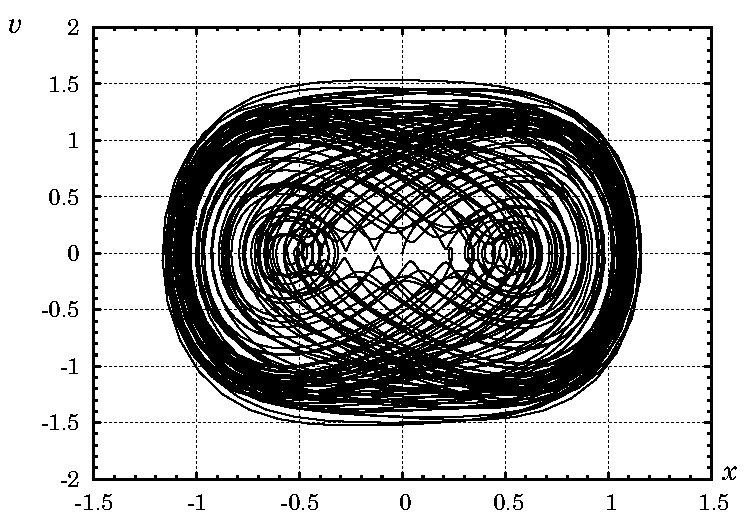
\includegraphics[width=0.5\textwidth]{p/cha/duff_phase.pdf} }
\caption{Фазовый портрет системы Дуффинга (\ref{atu:eq:duff})}
\label{atu:f:duff_phase}
\end{figure}

Критерий
$\overline{x^2}$

